\section{DICOM en pratique}

\frame
{
	\frametitle{Anonymisation}
	\begin{itemize}
		\item Utilisation d�images cliniques pour la recherche ou l�enseignement.
		\item Fichiers mis � disposition du public.
		\item N�cessit� d�anonymat : suppression des informations personnelles permettant d'identifier le patient.
		\begin{itemize}
			\item PatientsName (0010,0010)
			\item PatientID (0010,0020)
			\item PatientBirthDate (0010,0030)
			
			$\rightarrow$ de type 1 : � remplacer, pas supprimer !
			\item ReferringPhysicianName (0008,0090)
			\item etc.
		\end{itemize}
	\end{itemize}
}

\frame
{
	\frametitle{Achat d'un �quipement}
	\begin{enumerate}
		\item Avant l'achat : soumission de l'appel d'offre
		\begin{itemize}
			\item D�finition du sc�nario de travail souhait�.
			
			Exemple : les images brutes export�es pourront �tre r�utilis�es a posteriori.
			\item R�daction du cahier des charges DICOM.
			\begin{itemize}
				\item Pr�ciser le niveau d�exigence de DICOM.
				
				$\rightarrow$ faire appel � un consultant ou � des coll\'egues,
				
				$\rightarrow$ ou acqu�rir le savoir-faire en interne.
				\item Demander le Document de Conformit� DICOM.
			\end{itemize}
		\end{itemize}
		\item Acceptation protocol�e.
		\begin{itemize}
			\item V�rification de DICOM.
			\item V�rification des du sc�narios requis.
			\item Tests.
		\end{itemize}
	\end{enumerate}
}

\frame
{
	\frametitle{DICOM Conformance}
	Point faible abord� rapidement la derni\'ere fois.
	\begin{itemize}
		\item Le standard pr\'evoit un document "DICOM Conformance Statement" dont le plan et la structure sont pr\'ed\'efinis.
		\item Par ce document, le fournisseur pr\'ecise le niveau de conformit\'e de son \'equipement au standard DICOM.
		\begin{itemize}
			\item Applicable sur chaque mod\`ele, chaque version.
			\item Le document suit un plan pr\'evu dans le standard.
			\item Liste des SOP Class support\'ees et des r�les assur\'es (SCU, SCP).
		\end{itemize}
	\end{itemize}
}

\frame
{
	\frametitle{Services � demander}
	Exemples typiques de services DICOM � exiger pour un scanner :
	\begin{itemize}
		\item Worklist (SCU) : Import de la liste de patients.
		\item Store : envoi des images par r�seau
		\begin{itemize}
			\item Envoi : modalit�s (SCU) : \textbf{CT}.
			\item R�ception (SCP) : \textbf{CT}, \textbf{IRM}.
		\end{itemize}
		\item Print (SCU) : envoi des images pour impression
	\end{itemize}
	
	\begin{center}
		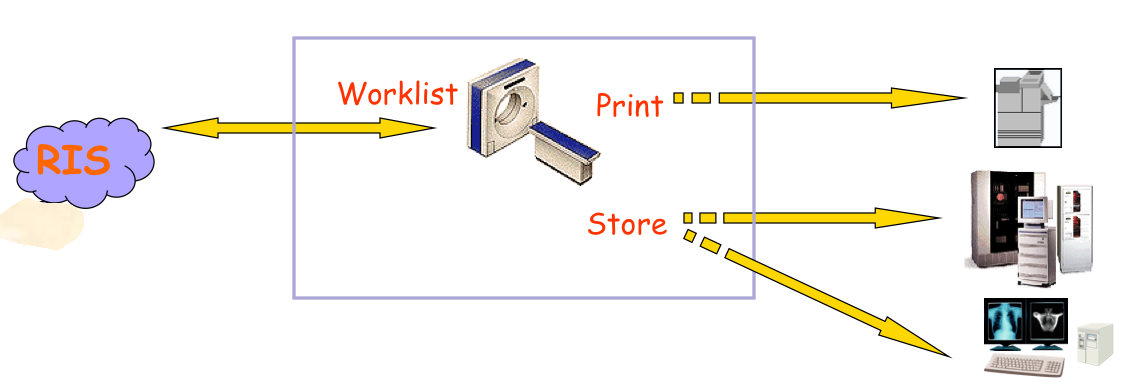
\includegraphics[width=\linewidth]{./figures/services-ct.png}
	\end{center}

}

\frame
{
	\frametitle{�quipements non standards}
	
	\begin{itemize}
		\item Int�grer dans un workflow DICOM : installer une passerelles de conversion.
		
		\begin{center}
			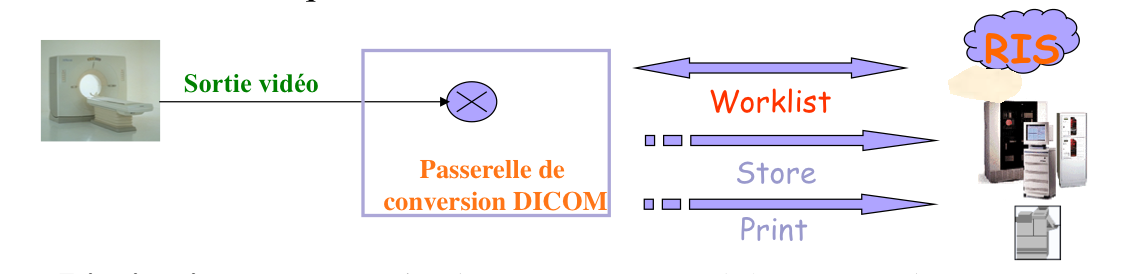
\includegraphics[width=\linewidth]{./figures/passerelle.png}
		\end{center}
		\item Limitation : images stock�es en mode Secondary Capture (IOD le plus simple de DICOM), les donn�es d'acquisition des images sont perdues.
	\end{itemize}
}
